\chapter[O Tribunal de Contas da União]{O Tribunal de Contas da União}

\section{História}
O TCU é um orgão adminstrativo autônomo e independetente que auxilia o Congresso Nacional (CN) em realizar o controle externo dos recursos públicos federais \cite{TCUHistoria}. Além disso o orgão possui sede em Brasília no Distrito Federal (DF) e jurisdição em todo território nacional \cite{Art73}. 

A instituição teve seu surgimento pela Constituição de \textbf{1891}, sob influência de Rui Barbosa, institucionalizou definitivamente o TCU, mas sua instalação só ocorreu em 17 de janeiro de \textbf{1893}, graças ao emprenho do Ministro da Fazenda Serzedello Corrêa  do governo de Floriano Peixoto \cite{TCUHistoriaJUS}. Logo, o TCU teve a competência para exame, revisão e julgamento de todas as operações relacionadas com a receita e a despesa da União. Nos anos seguintes as responsabilidades do TCU foram acrescentadas\cite{TCUHistoriaJUS}:

\begin{itemize}
	\item \textbf{1937:} Com exceção do parecer sobre as contas da presidência, todas as atribuições ao tribunal foram mantidas;
	
	\item \textbf{1946:} Acrescentou o julgamento a legalidade das concessões de aponsentadorias, reformas e pensões;
	
	\item \textbf{1967:} De acordo com a Constituição de \textbf{1967}, retirou do TCU o exame e julgamento prévio dos atos e dos contratos geradores de despesas, sem prejuízo da competência para apontar falhas e irregularidades; 
\end{itemize}

Então de acordo com Luiz Eduardo Oliveira Alejarra, no ano de \textbf{1988} o TCU passou a obter: 

\begin{citacao}
	o Tribunal de Contas da União teve a sua jurisdição e competência substancialmente ampliadas. Recebeu poderes para, no auxílio ao Congresso Nacional, exercer a fiscalização contábil, financeira, orçamentária, operacional e patrimonial da União e das entidades da administração direta e indireta, quanto à legalidade, à legitimidade e à economicidade e a fiscalização da aplicação das subvenções e da renúncia de receitas. Qualquer pessoa física ou jurídica, pública ou privada, que utilize, arrecade, guarde, gerencie ou administre dinheiros, bens e valores públicos ou pelos quais a União responda, ou que, em nome desta, assuma obrigações de natureza pecuniária tem o dever de prestar contas ao TCU \cite[p. 1]{TCUHistoriaJUS}.
\end{citacao}

\pagebreak

\section{Logo}

A logo atual do Tribunal de Contas é apresentada pela figura \ref{logoTCU}.  

\begin{figure}[h!]
	\centering
	
\includegraphics[keepaspectratio=true,scale=0.5]{figuras/TCU.jpg}
	\caption{Logo do TCU. Fonte: \cite{TCUHistoria}}
	\label{logoTCU}
\end{figure}

\section{Endereço}

O endereço da sede do TCU onde o estágio exerceu as atividades:
St. de Administração Federal Sul, Quadra:4 Lote:01 - Asa Sul, Brasília - DF, 70042-900 \cite{TCUHistoria}



\chapter[Atividades Desenvolvidas e Cronograma de Execução]{Atividades Desenvolvidas e Cronograma de Execução}

Neste Cápitulo é apresentado as atividades desenvolvidas de acordo com o Plano de Atividades, anexado ao Termo Aditivo do Contrato. A descrição das atividades que foram propostas a serem desenvolvidas e a carga horária semanal é apresentada na tabela \ref{AtividadesDaPA} 

\begin{table}[h]
	\centering
	\caption{Descrição das atividades propostas no Plano de Atividades}
	\label{AtividadesDaPA}
	\begin{tabular}{|c|c|c|}
		\hline
		\textbf{Identificador} & \textbf{Atividade} & \textbf{\begin{tabular}[c]{@{}c@{}}Carga horária\\ Semanal\end{tabular}} \\ \hline
		1 & \begin{tabular}[c]{@{}c@{}}Auxiliar no desenvolvimento de sistemas em\\ Oracle Application Express, abrangendo as \\ atividades de levantamento de requisitos,\\ modelagem de banco de dados, implementação,\\ teste, documentação e manutenção\end{tabular} & 4h \\ \hline
		2 & Auxiliar a manutenção de sistemas (Sidarq) & 10h \\ \hline
		3 & Auxiliar organização de sistemas & 5h \\ \hline
		4 & Auxiliar as áreas de suporte & 1h \\ \hline
	\end{tabular}
\end{table}

A Figura \ref{Cronograma} apresenta o cronograma de atividades realizado pelo estagiário durante o período do contrato.

\begin{figure}[h!]
	\centering
	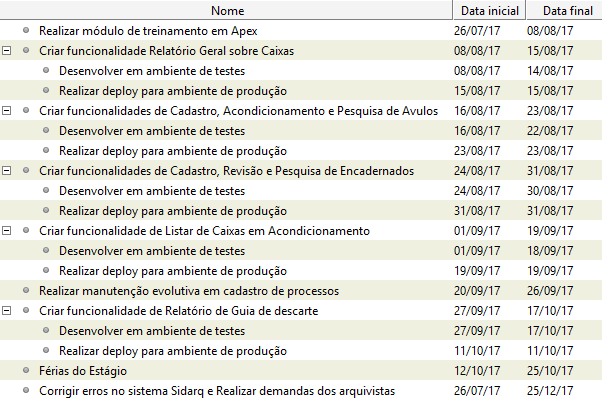
\includegraphics[keepaspectratio=true,scale=0.8]{figuras/Cronograma.PNG}
	\caption{Cronograma Geral de Atividades.}
	\label{Cronograma}
\end{figure}

\chapter[Resultados e Discussão]{Resultados e Discussão}

Como resultados das atividades já realizadas o Sidarq atingiu sua primeira versão estável (\textbf{V1.0.0}) e que atualmente está em ambiente de produção, sendo utilizada pelos arquivistas do CDOC.

\begin{itemize}
	\item Funcionalidades implementas pelo estagiário.
	\begin{todolist}
		\item[\done] Relatório Geral Sobre Caixas;
		\item[\done] Cadastro de Avulsos;
		\item[\done] Acondicionamento de Avulsos;
		\item[\done] Pesquisa de Avulsos;
		\item[\done] Cadastro de Encadernados;
		\item[\done] Lista de Caixas em Acondicionamento;
		\item[\done] Inserção de Link do E-TCU no Cadastro de Processos;
		\item[\done] Relatório de Guia de Descarte;
	\end{todolist}
\end{itemize}

Em termos de manutenção corretiva foi aplicado ao Sidarq as correções de \textit{bugs} de acordo com o Apex, os erros que não possuem marcação significam que o estagiário, não aplicou nenhuma correção do tipo: 

\begin{itemize}
	\item Erros:
	\begin{todolist}
		\item[\done] Referências com sintaxe de substituição;
		\item[\done] Referências com sintaxe de coluna;
		\item[\done] Referências com Bind Variable Syntax;
		\item[\done] Referências Declarativas de Itens de Aplicação, Itens de Página, Colunas ou Filtros de Relatório Interativo;
		\item[\done] Existe um número de página de referência;
		\item[\done] O código válido SQL ou PL / SQL;
		\item[\done] Fetch, DML, MR * Os processos são válidos
		\item Ramo incondicional antes de outros ramos;
		\item[\done] Botão Referenciado no Botão Quando Pressionado existe;
		\item[\done] O botão não é compatível com ações dinâmicas;
	\end{todolist}
	
	\item Segurança:
	\begin{todolist}
		\item[\done] Uso inapropriado da sintaxe de substituição;
		\item[\done] Atributos do aplicativo que podem ser bloqueados;
		\item[\done] Autorização;
		\item[\done] Proteção do Estado de Sessão;
		\item[\done] Configurações de segurança do navegador;
	\end{todolist}

	\item Warnings:
	\begin{todolist}
		\item[\done] Item referenciado está na página atual;
		\item[\done] O item referenciado é Item da página da página de destino;
		\item[\done] Referências de Item da Página em uma Cadeia de Caracteres;
		\item[\done] Comprimento do item ou nome da coluna do formulário tabular;
		\item[\done] Referências inconsistentes entre ações dinâmicas e botões;
		\item[\done] Itens protegidos em chamadas AJAX;
	\end{todolist}

    \item Performance:
    \begin{todolist}
    	\item[\done] Função V usada em instruções SQL;	
    \end{todolist}
    
    \item Usabilidade:
    \begin{todolist}
    	\item[\done] A Autorização da página de destino também está configurada para componente atual;
    	\item[\done] Item Associado ou Coluna de Validações;
	\end{todolist}


	\item Garantia da Qualidade:
	\begin{todolist}
		\item[\done] ID do aplicativo codificado;
		\item[\done] O Relatório tem Ordem Padrão;
		\item[\done] Item da página tem texto de ajuda;
		\item[\done] Valores de atributo depreciados;
	\end{todolist}
\end{itemize}

Com base no proposto no plano de atividades as atividades foram executadas com sucesso e com satisfação e aprovação, tanto pelos usuários do Sidarq quanto pelo Supervisor. Atualmente as atividades realizadas, são atividades de correção de bugs, seguindo o checklist que já foi satisfeito em várias partes da aplicação.

\chapter[Considerações Finais]{Considerações Finais}

